\documentclass[11pt,a4paper]{article}

\usepackage[T1]{fontenc}
\usepackage[utf8]{inputenc}
\usepackage{mathpazo}
\usepackage[scaled=0.92]{helvet}
\renewcommand{\ttdefault}{lmtt}
\usepackage[margin=2.4cm]{geometry}
\usepackage{amsmath}
\usepackage{graphicx}
\usepackage{booktabs}
\usepackage{array}
\usepackage{enumitem}
\usepackage{tikz}
\usetikzlibrary{arrows.meta,positioning,calc}
\usepackage{xcolor}
\usepackage{longtable}
\usepackage{tabularx}
\usepackage{titlesec}
\usepackage{fancyhdr}
\usepackage[colorlinks=true,linkcolor=black,citecolor=black,citecolor=black,urlcolor=blue!50!black]{hyperref}

\graphicspath{{figures/}}
\setlength{\parindent}{0pt}
\setlength{\emergencystretch}{2em}
\setlength{\parskip}{0.5em}
\setlist{itemsep=0.15em,topsep=0.2em}
\renewcommand{\arraystretch}{1.25}

\titleformat{\section}{\Large\bfseries\sffamily}{\thesection}{0.6em}{}
\titleformat{\subsection}{\large\bfseries\sffamily}{\thesubsection}{0.6em}{}
\titlespacing*{\section}{0pt}{1.6em}{0.5em}
\titlespacing*{\subsection}{0pt}{1.1em}{0.3em}

\pagestyle{fancy}
\fancyhf{}
\fancyhead[L]{\small\sffamily Multimodal fusion: the theory you need}
\fancyhead[R]{\small\sffamily\thepage}
\renewcommand{\headrulewidth}{0.3pt}

% "Where it is used" line under a section title
\newcommand{\usedin}[1]{{\small\sffamily\color{black!60}Used in: #1}\par\vspace{0.2em}}
% Key term
\newcommand{\term}[1]{\textbf{#1}}
% Code
\newcommand{\code}[1]{\texttt{\small #1}}
% A short framed summary at the end of a section
\newcommand{\remember}[1]{%
  \par\vspace{0.4em}\noindent\fcolorbox{black!35}{black!4}{\parbox{\dimexpr\linewidth-2\fboxsep-2\fboxrule}{%
  \textbf{\sffamily Remember.} #1}}\par}
% A framed warning
\newcommand{\careful}[1]{%
  \par\vspace{0.4em}\noindent\fcolorbox{black!35}{black!4}{\parbox{\dimexpr\linewidth-2\fboxsep-2\fboxrule}{%
  \textbf{\sffamily Careful.} #1}}\par}

% Diagram styles (same language for all the diagrams)
\definecolor{fusionteal}{RGB}{13,145,130}
\tikzset{
  dat/.style={draw, fill=black!8, minimum height=0.75cm, minimum width=2.5cm, align=center, font=\footnotesize\sffamily},
  mod/.style={draw, fill=fusionteal!22, minimum height=0.75cm, minimum width=2.5cm, align=center, font=\footnotesize\sffamily},
  jn/.style={draw, thick, fill=white, minimum height=0.75cm, minimum width=2.5cm, align=center, font=\footnotesize\sffamily},
  arr/.style={-{Stealth[length=2mm]}, thick}
}

% Part heading: new page, big title, one sentence
\newcommand{\parthead}[3]{\clearpage
  {\noindent\small\sffamily\color{fusionteal}\textbf{#1}}\\[0.1em]
  {\noindent\LARGE\bfseries\sffamily #2}\\[0.3em]
  {\noindent\small\itshape #3}\par
  \vspace{0.2em}\noindent{\color{fusionteal}\rule{\linewidth}{0.8pt}}\par}
% Closing list of readings
\newcommand{\further}[1]{\par\vspace{0.5em}\noindent{\small\sffamily\bfseries To study further}\par
  \begin{itemize}[leftmargin=1.4em,itemsep=0.1em,topsep=0.1em]\small #1\end{itemize}}
% Optional box "How to use"
\newcommand{\howto}[1]{\par\noindent\fcolorbox{fusionteal}{fusionteal!6}{\parbox{\dimexpr\linewidth-2\fboxsep-2\fboxrule}{#1}}\par}
\tikzset{
  tag/.style={font=\footnotesize\sffamily\bfseries, anchor=south west}
}
\begin{document}

\begin{center}
{\LARGE\bfseries\sffamily Multimodal fusion}\\[0.4em]
{\Large\sffamily Images and clinical data together: the theory you need}\\[0.8em]
{\small MSc Health Informatics, Advanced Topics in Machine Learning}\\[0.2em]
{\small Optional module. Version: academic year 2026/27}
\end{center}

\vspace{0.6em}

\howto{\textbf{\sffamily How to use this handbook.}
\begin{itemize}[leftmargin=1.4em,itemsep=0.05em,topsep=0.2em]
\item Read it next to the notebook: every chapter says which STEP it supports.
\item Chapters 1 to 4 and 6 to 7 are the core. Chapter 5 (embeddings) goes with STEP 8 and the challenges at the end.
\item Each chapter ends with a \emph{Remember} box and a short list of readings. Numbers in square brackets point to the References.
\item The clinical data are \textbf{invented}. Only the images are real.
\end{itemize}}

\vspace{0.8em}

\begin{center}
\small
\begin{tabular}{@{}rp{6.6cm}lr@{}}
\toprule
Chapter & Topic & Used in & Page \\
\midrule
\multicolumn{4}{@{}l}{\sffamily\bfseries Part I. The setting}\\
1 & Why more than one kind of data & Introduction & \pageref{c:1}\\
2 & The data of this module & STEP 1--2 & \pageref{c:2}\\
3 & Measuring a model on patients & STEP 3--4 & \pageref{c:3}\\
\addlinespace
\multicolumn{4}{@{}l}{\sffamily\bfseries Part II. From an image to numbers}\\
4 & Measurements from a mask & STEP 5 & \pageref{c:4}\\
5 & Embeddings & STEP 8 and challenges & \pageref{c:5}\\
\addlinespace
\multicolumn{4}{@{}l}{\sffamily\bfseries Part III. Putting the sources together}\\
6 & Three ways to fuse & STEP 6, 7 and 9 & \pageref{c:6}\\
7 & Reading the results & STEP 10 & \pageref{c:7}\\
8 & Outside this notebook & Reading & \pageref{c:8}\\
\addlinespace
 & References & & \pageref{c:refs}\\
 & Index of terms & & \pageref{c:index}\\
\bottomrule
\end{tabular}
\end{center}

% ===========================================================================
\parthead{Part I}{The setting}{What we want to know, what data we have, and how to measure an answer fairly.}

\section{Why more than one kind of data}\label{c:1}

A \term{modality} is one kind of data: a CT image, a table of laboratory values, a report written by a
radiologist. A doctor rarely decides from one modality. Looking at a nodule on a CT, the doctor also asks how old
the patient is, whether the patient smokes, and how well the patient manages daily life. Each source tells
something that the others do not. Medicine is multimodal by nature \cite{acosta2022multimodal,lipkova2022multimodal}.

\term{Multimodal fusion} means building one model that uses several modalities. It is a whole field of machine
learning, not only a medical topic \cite{baltrusaitis2019multimodal}.

\begin{center}
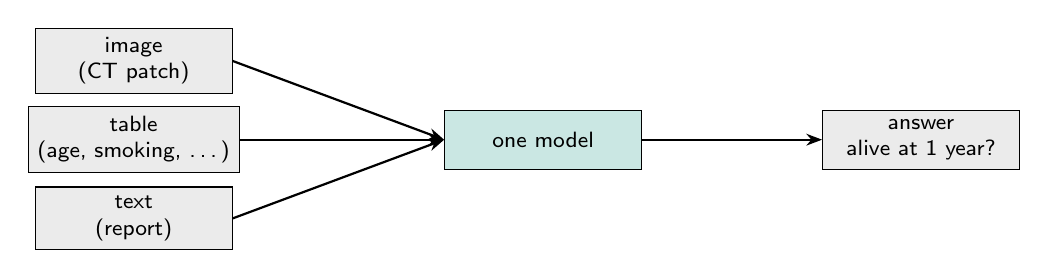
\begin{tikzpicture}
\node[dat] (a) at (0,1.0) {image\\(CT patch)};
\node[dat] (b) at (0,0) {table\\(age, smoking, \dots)};
\node[dat] (c) at (0,-1.0) {text\\(report)};
\node[mod] (m) at (5.2,0) {one model};
\node[dat] (o) at (10,0) {answer\\alive at 1 year?};
\draw[arr] (a.east) -- (m.west);
\draw[arr] (b.east) -- (m.west);
\draw[arr] (c.east) -- (m.west);
\draw[arr] (m) -- (o);
\end{tikzpicture}

{\small Fusion: several sources, one model, one answer. In this module we use the image and the table.}
\end{center}

The question of the module is simple: \emph{does a model that sees both the image and the clinical data predict
better than a model that sees only one of them?} You will find the answer by measuring, and the handbook explains
how to do it without fooling yourself.

\remember{A modality is a kind of data. Fusion is one model that reads more than one. The module asks whether
fusion beats the best single source.}

\further{
\item Acosta et al.\ \cite{acosta2022multimodal}: an overview of multimodal AI in biomedicine.
\item Lipkova et al.\ \cite{lipkova2022multimodal}: the same idea seen from oncology.
\item Baltru\v{s}aitis et al.\ \cite{baltrusaitis2019multimodal}: the survey that organises the whole field.
}

% ---------------------------------------------------------------------------
\section{The data of this module}\label{c:2}
\usedin{notebook STEP 1--2}

The images are real. They are the nodule patches of notebook 04, cut from the LUNA16 chest CT collection
\cite{setio2017luna16}: $64 \times 64$ pixels around a nodule, with the mask of the nodule. For this module we
keep one nodule per patient, the largest, so we have 601 patients.

\begin{center}
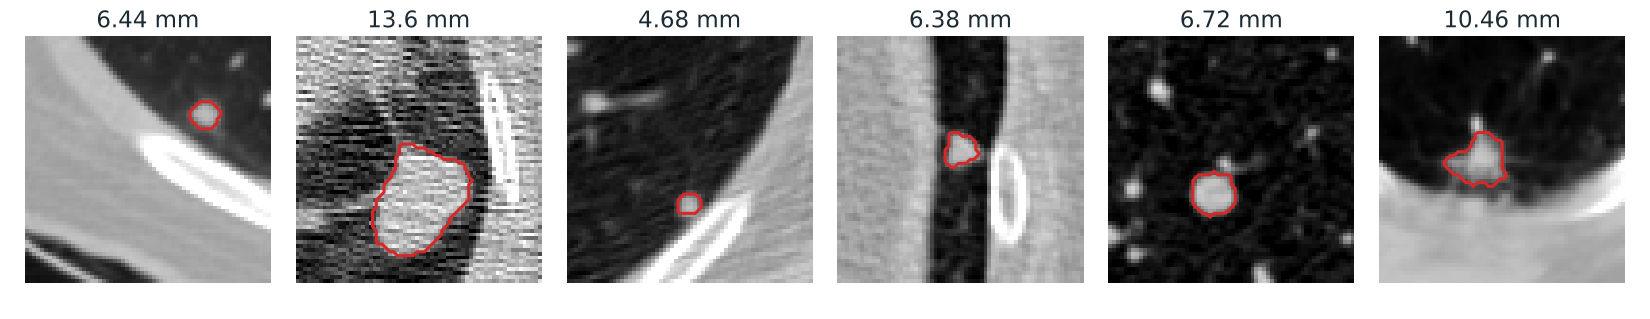
\includegraphics[width=0.9\linewidth]{fusion_patches.png}

{\small Six patches, with the border of the mask in red. The title of each is the diameter of the nodule.}
\end{center}

Real clinical data cannot be shared in a course, so the clinical table is generated by a formula, and so is the
outcome we want to predict, \code{alive\_1y}. You have a table with one row per patient:

\begin{center}
\small
\begin{tabular}{@{}lp{6.4cm}l@{}}
\toprule
Column & Meaning & Origin \\
\midrule
\code{age}, \code{sex} & age in years, F or M & invented \\
\code{pack\_years} & smoking history: packs per day times years & invented \\
\code{performance\_status} & 0 fully active, 1 some limits, 2 in bed part of the day & invented \\
\code{alive\_1y} & \textbf{the target}: 1 alive one year later, 0 not & invented, from a formula \\
\bottomrule
\end{tabular}
\end{center}

\careful{The clinical data and the outcome are invented. The formula uses the size and the density of the real
nodule, plus age, performance status and smoking. Nothing here has a medical meaning: the point is the method.
The notebook shows you the formula at the end.}

In the table the fraction of patients alive after one year is 0.697.

\remember{Real images, invented table, invented outcome. Whatever you find is a statement about the method, not
about lung cancer.}

\further{
\item Setio et al.\ \cite{setio2017luna16}: the LUNA16 challenge, the source of the images.
\item MONAI documentation \cite{monaidocs}: how medical images are read and prepared in the course.
}

% ---------------------------------------------------------------------------
\section{Measuring a model on patients}\label{c:3}
\usedin{notebook STEP 3--4}

\textbf{The split.} The model learns on the \term{training} patients and is judged on the \term{test} patients,
whom it has never seen. We use 420 for training and 181 for testing, with the same fraction of alive patients in
both (\code{stratify=y}).

\begin{center}
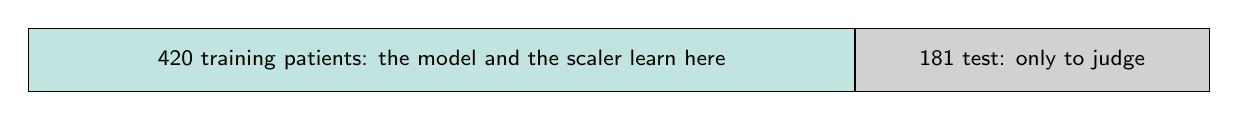
\begin{tikzpicture}
\fill[fusionteal!25] (0,0) rectangle (10.5,0.8);
\fill[black!18] (10.5,0) rectangle (15,0.8);
\draw (0,0) rectangle (15,0.8);
\draw (10.5,0) -- (10.5,0.8);
\node[font=\footnotesize\sffamily] at (5.25,0.4) {420 training patients: the model and the scaler learn here};
\node[font=\footnotesize\sffamily] at (12.75,0.4) {181 test: only to judge};
\end{tikzpicture}

{\small The 601 patients, split once. Every model of the module uses this split.}
\end{center}

\textbf{The AUC.} The model gives each test patient a probability of being alive. The \term{AUC} is the
probability that a patient who was alive gets a higher score than a patient who was not. You know it from the
first year; three lines are enough:
\begin{itemize}
\item 0.5 is a coin toss;
\item 1.0 is a perfect ordering of the patients;
\item it does not depend on a threshold, so it compares models that have different probabilities.
\end{itemize}

\textbf{One test set for all.} Every model of the module is judged on the same 181 test patients, through the
same function \code{test\_auc}. If each model had its own test patients, a difference could come from the patients
and not from the model.

\textbf{Baselines first.} We start with a model on the clinical data only (STEP 4) and a model on the image
only. They are the \term{baselines}. A fusion model is useful only if it beats the best of them. If you skip the
baselines, you cannot say whether fusion helped.

\textbf{Fit on the training patients only.} Anything that learns from data, such as a scaler or a PCA, must be
fitted on the training patients and then applied to the test patients. If the test patients take part in any
step of the learning, the AUC is too good and will not hold on new patients. This is called \term{leakage}, and
it is a common reason why published results fail to reproduce \cite{kapoor2023leakage}.

\remember{Same split, same metric, the single-modality models first, and everything that learns is fitted on the
training patients only.}

\further{
\item Kapoor and Narayanan \cite{kapoor2023leakage}: how leakage enters a study and how to spot it.
\item Chapter 7 of this handbook: what a small test set lets you say.
}

% ===========================================================================
\parthead{Part II}{From an image to numbers}{Our model reads a table, not pixels: two ways to turn a patch into columns.}

The model of this module is a logistic regression (except in STEP 9, where it is a small network). It reads a
table of numbers, not pixels. So the first job is to turn the patch into a few numbers. There are two ways, and
the notebook tries both.

\begin{center}
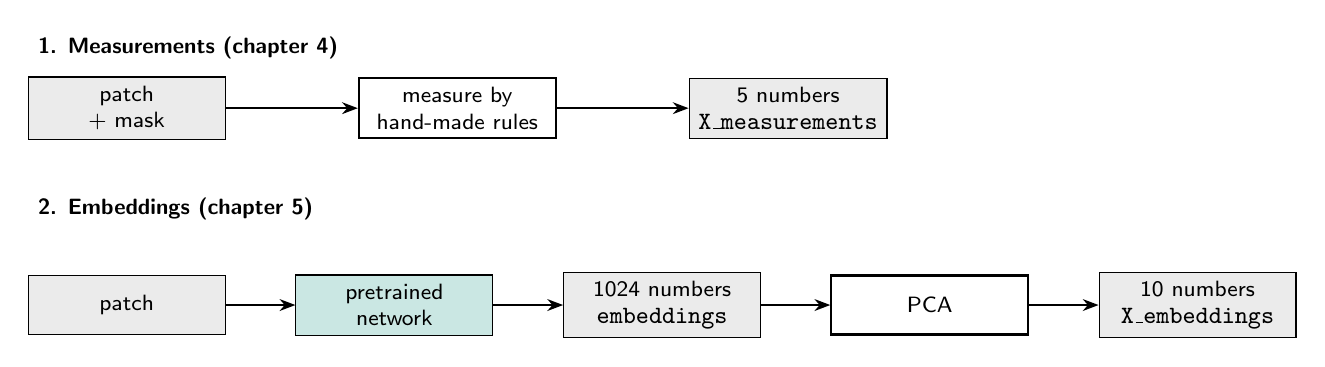
\begin{tikzpicture}[x=1cm,y=1cm]
\node[dat] (p1) at (0,0) {patch\\+ mask};
\node[jn]  (m1) at (4.2,0) {measure by\\hand-made rules};
\node[dat] (n1) at (8.4,0) {5 numbers\\\code{X\_measurements}};
\draw[arr] (p1) -- (m1);
\draw[arr] (m1) -- (n1);
\node[tag] at (-1.25,0.5) {1. Measurements (chapter 4)};
\node[dat] (p2) at (0,-2.5) {patch};
\node[mod] (m2) at (3.4,-2.5) {pretrained\\network};
\node[dat] (n2) at (6.8,-2.5) {1024 numbers\\\code{embeddings}};
\node[jn]  (m3) at (10.2,-2.5) {PCA};
\node[dat] (n3) at (13.6,-2.5) {10 numbers\\\code{X\_embeddings}};
\draw[arr] (p2) -- (m2);
\draw[arr] (m2) -- (n2);
\draw[arr] (n2) -- (m3);
\draw[arr] (m3) -- (n3);
\node[tag] at (-1.25,-1.55) {2. Embeddings (chapter 5)};
\end{tikzpicture}
\end{center}

\section{Measurements from a mask}\label{c:4}
\usedin{notebook STEP 5}

The mask tells us where the nodule is. With it we measure, as a radiologist would do with a ruler.
The \term{area} is the number of pixels of the mask times the \term{pixel spacing} (in mm) along $x$ and $y$.
From the area we take the diameter of the circle with the same area:
\[
d = 2\sqrt{A/\pi}.
\]
Then we read the Hounsfield values of the pixels inside the mask, and keep their mean, their standard deviation
(how much they vary) and their maximum. That gives five numbers: area, diameter, mean, standard deviation and
maximum, which is the table \code{X\_measurements}.

\begin{center}
\begin{minipage}[c]{0.36\linewidth}
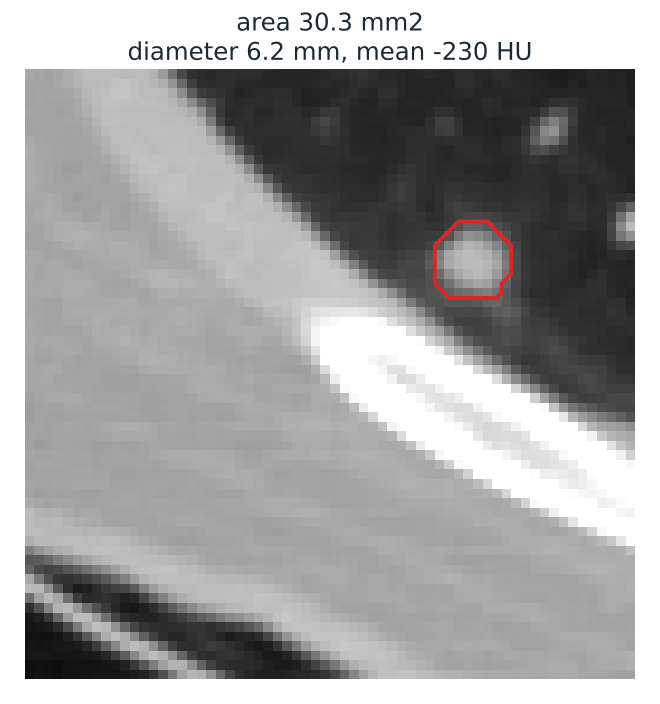
\includegraphics[width=\linewidth]{fusion_measure.png}
\end{minipage}\hfill
\begin{minipage}[c]{0.60\linewidth}
Patient 0, the example of STEP 5. The mask has an area of 30.30 mm$^2$, which gives a diameter of 6.21 mm; the
metadata of the dataset says 6.44 mm. Inside the mask the mean is $-230.5$ HU, the standard deviation 179.1 HU
and the maximum 28 HU.
\end{minipage}
\end{center}

\subsection*{Radiomics}

This is the idea of \term{radiomics}: describe a lesion by numbers, so that images become data
\cite{gillies2016radiomics,lambin2012radiomics}. The numbers fall in three families.
\begin{itemize}
\item \textbf{Shape}: size, roundness, how irregular the border is.
\item \textbf{Intensity}: the statistics of the Hounsfield values inside the mask.
\item \textbf{Texture}: how the values are arranged in space, smooth or patchy.
\end{itemize}
We use the simplest ones, one from each of the first two families. The usual software is PyRadiomics
\cite{vangriethuysen2017pyradiomics}, which computes many of them. Because the same name can hide different
computations in different programs, an international effort works to standardise the features
\cite{zwanenburg2020ibsi}.

\textbf{Strength:} few numbers, and each one means something you can explain to a clinician.
\textbf{Limit:} somebody chooses them. A property nobody thought of is not measured.

\careful{The numbers depend on the mask: a different person, or a different program, draws a different border, and
the area changes. They also depend on the scanner and the software: the same nodule on two machines gives
slightly different values. Radiomics works best when masks and scanners are the same in training and in use.}

\remember{A mask gives a few meaningful numbers: size, mean density, spread. They are easy to explain and
depend on who draws the mask and on the scanner.}

\further{
\item Gillies et al.\ \cite{gillies2016radiomics} and Lambin et al.\ \cite{lambin2012radiomics}: the two papers that made radiomics a field.
\item PyRadiomics \cite{vangriethuysen2017pyradiomics}: the library; its documentation lists every feature \cite{pyradiomicsdocs}.
\item Zwanenburg et al.\ \cite{zwanenburg2020ibsi}: the standard definitions of the features.
}

% ---------------------------------------------------------------------------
\section{Embeddings}\label{c:5}
\usedin{notebook STEP 8 and the challenges at the end}

In chapter 4 we chose the numbers by hand. Here a network chooses them. This chapter is the longest because
the choices are many, and a wrong one is easy to make without noticing.

\subsection{What an embedding is}

A neural network that classifies an image turns it, layer after layer, into a list of numbers, and the last layer
turns that list into an answer. The list just before the answer is the \term{embedding} of the image. We stop
there and keep the list. We train nothing: the network was trained by somebody else, on another task, and we use
it as a measuring tool. This is the idea of representation learning \cite{bengio2013representation}: a good
list of numbers makes the next problem easy.

\begin{center}
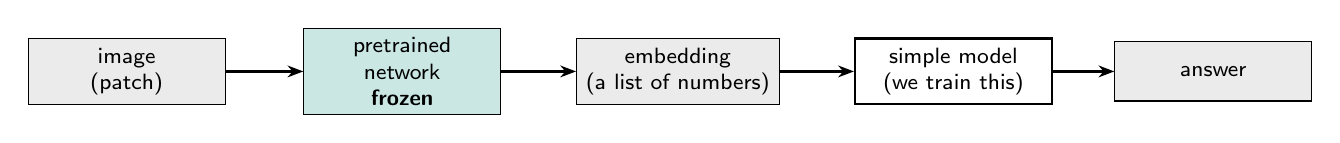
\begin{tikzpicture}
\node[dat] (a) at (0,0) {image\\(patch)};
\node[mod] (b) at (3.5,0) {pretrained\\network\\\textbf{frozen}};
\node[dat] (c) at (7,0) {embedding\\(a list of numbers)};
\node[jn]  (d) at (10.5,0) {simple model\\(we train this)};
\node[dat] (e) at (13.8,0) {answer};
\draw[arr] (a) -- (b);
\draw[arr] (b) -- (c);
\draw[arr] (c) -- (d);
\draw[arr] (d) -- (e);
\end{tikzpicture}

{\small We use the network up to the embedding, and learn only the small model on top.}
\end{center}

You can read an embedding as a description of the image written by the network, in a language we do not read.
In our notebook it has 1024 numbers (a DenseNet121 trained on ImageNet) and we reduce them to 10 with a PCA, so
that 420 patients are enough to learn from.

\subsection{What makes an embedding good}

Not every embedding is useful for your problem. For ours, a good one has seven properties.
\begin{enumerate}
\item \textbf{It keeps what the answer needs.} Here the risk depends on the size and on the density of the
nodule, so the embedding must contain them, even if nobody asked the network for them.
\item \textbf{It ignores what does not matter:} where the nodule sits in the patch, the noise of the scanner, the
vessels around. Be careful, because what a network was trained to ignore may be what you need. Networks trained
on photographs learn that an object is the same object when it is larger or smaller in the picture. For a
nodule the size is the message. This is a likely reason why measurements beat embeddings here, not a proven fact.
\item \textbf{It puts similar cases close together.} The nearest neighbours of a nodule are nodules that look
like it.
\item \textbf{It is easy to read.} A simple model on top, such as a logistic regression, is enough. With few
patients this is all you can afford.
\item \textbf{It comes from images like yours.} A network that has only seen photographs has never seen a CT.
Whether pretraining on photographs helps in medicine is debated \cite{raghu2019transfusion}, and networks
pretrained on medical images exist \cite{mei2022radimagenet}.
\item \textbf{It is not too large for your number of patients.} 1024 numbers for 420 patients must be reduced or
regularised.
\item \textbf{It is stable.} A small change of the crop or of the window should change it little.
\end{enumerate}

\textbf{How to check, before you trust it.} Four checks, from the cheapest.
\begin{itemize}
\item \textbf{A probe.} Can a simple model predict from the embedding something you already know, such as the
diameter? We do it in section 5.6: it is the column $R^2$.
\item \textbf{The neighbours.} For a few nodules, look at the closest ones in embedding space. Do they look alike?
\item \textbf{A map.} Draw two PCA components, coloured by a known property. This is the figure of STEP 8.
\item \textbf{The task itself}, always next to a baseline: the five measurements and the clinical data alone.
\end{itemize}

\begin{center}
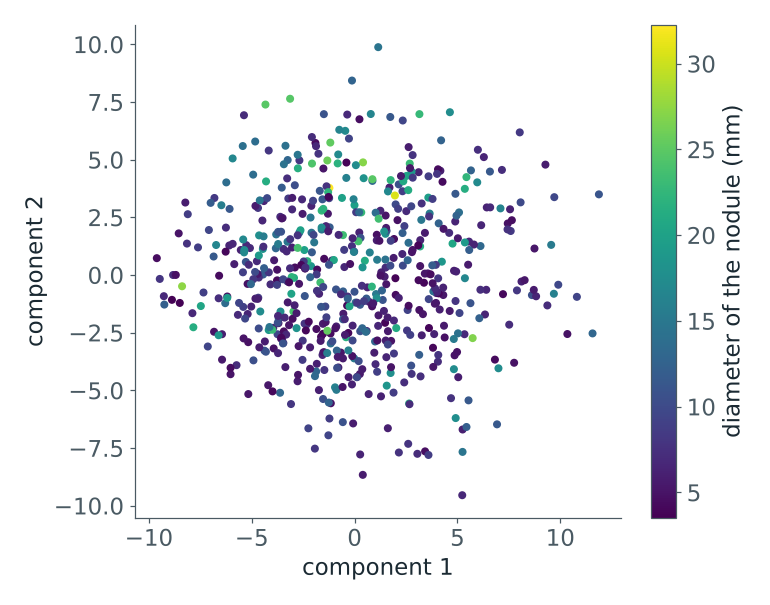
\includegraphics[width=0.32\linewidth]{fusion_pca.png}

{\small The first two PCA components of the 601 patches. The colour is the diameter of the nodule. The colours
are mixed: the two components know only a little about the size.}
\end{center}

\subsection{Three recipes to train the network}

An embedding is as good as the way its network was trained. There are three recipes, and every model of the next
section follows one of them.

\begin{center}
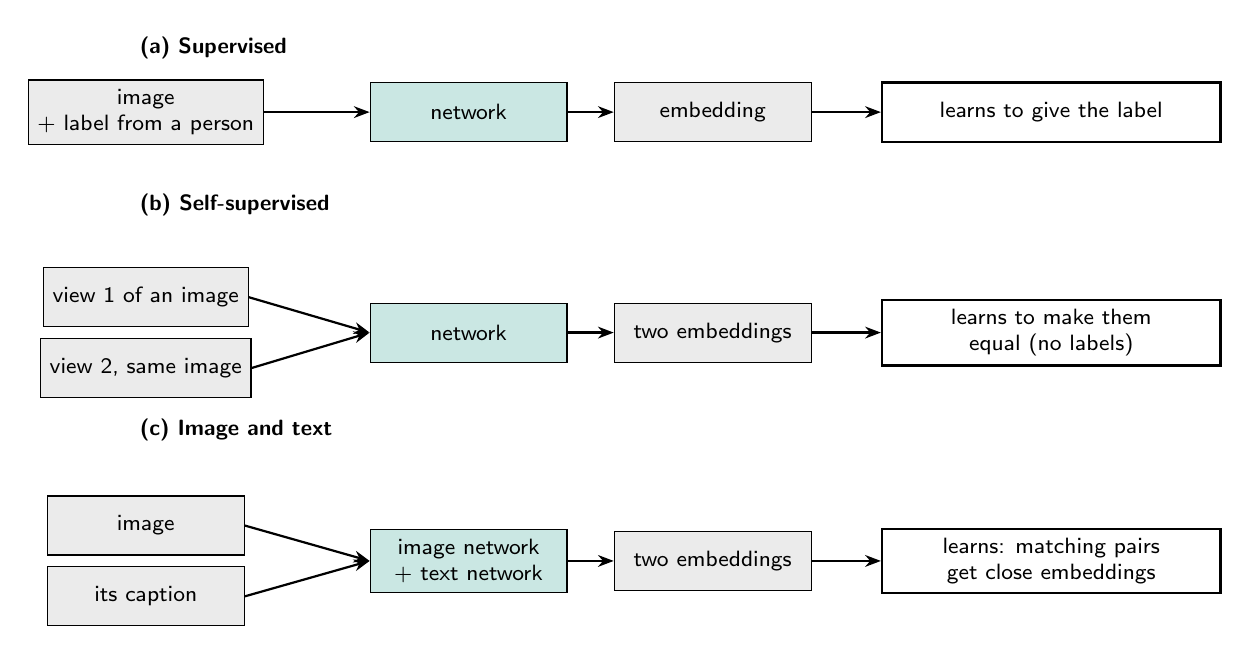
\begin{tikzpicture}[x=1cm,y=1cm]
\tikzset{wide/.style={draw, thick, fill=white, minimum height=0.75cm, minimum width=4.3cm, align=center, font=\footnotesize\sffamily}}
% a
\node[tag] at (-0.2,0.55) {(a) Supervised};
\node[dat] (a1) at (0,0) {image\\+ label from a person};
\node[mod] (a2) at (4.1,0) {network};
\node[dat] (a3) at (7.2,0) {embedding};
\node[wide] (a4) at (11.5,0) {learns to give the label};
\draw[arr] (a1) -- (a2); \draw[arr] (a2) -- (a3); \draw[arr] (a3) -- (a4);
% b
\node[tag] at (-0.2,-1.45) {(b) Self-supervised};
\node[dat] (b1) at (0,-2.35) {view 1 of an image};
\node[dat] (b2) at (0,-3.25) {view 2, same image};
\node[mod] (b3) at (4.1,-2.8) {network};
\node[dat] (b4) at (7.2,-2.8) {two embeddings};
\node[wide] (b5) at (11.5,-2.8) {learns to make them\\equal (no labels)};
\draw[arr] (b1.east) -- (b3.west); \draw[arr] (b2.east) -- (b3.west);
\draw[arr] (b3) -- (b4); \draw[arr] (b4) -- (b5);
% c
\node[tag] at (-0.2,-4.3) {(c) Image and text};
\node[dat] (c1) at (0,-5.25) {image};
\node[dat] (c2) at (0,-6.15) {its caption};
\node[mod] (c3) at (4.1,-5.7) {image network\\+ text network};
\node[dat] (c4) at (7.2,-5.7) {two embeddings};
\node[wide] (c5) at (11.5,-5.7) {learns: matching pairs\\get close embeddings};
\draw[arr] (c1.east) -- (c3.west); \draw[arr] (c2.east) -- (c3.west);
\draw[arr] (c3) -- (c4); \draw[arr] (c4) -- (c5);
\end{tikzpicture}
\end{center}

\textbf{(a) Supervised.} Images come with a label written by a person, and the network learns to give the label.
The classic case is ImageNet, about 1.3 million photographs in 1000 classes \cite{deng2009imagenet}. Networks such
as ResNet \cite{he2016resnet} and DenseNet \cite{huang2017densenet} are trained like this. Better ImageNet models
tend to transfer better to other photographs \cite{kornblith2019transfer}; for medical images the benefit is
debated \cite{raghu2019transfusion}. The same recipe on medical images gives RadImageNet \cite{mei2022radimagenet}
(CT, MRI and ultrasound) and, for volumes, Med3D \cite{chen2019med3d}. The cost is the label: somebody had to write
it for every image.

\textbf{(b) Self-supervised.} No labels. We make two different views of the same image and ask the network to give them the same embedding, and different embeddings to different images. This is
SimCLR \cite{chen2020simclr}. DINO \cite{caron2021dino} lets a student network match a teacher on different crops of
the same image, with Vision Transformers \cite{dosovitskiy2021vit}. DINOv2 \cite{oquab2023dinov2} is the same family
trained on 142 million photographs and made to be used frozen. Masked autoencoders \cite{he2022mae} hide most of the
image and learn to rebuild it. In medicine, self-supervised pretraining on medical images improves classification
\cite{azizi2021selfsup}, and there are models for chest X-rays \cite{perezgarcia2025raddino}, for lesions in CT
\cite{pai2024foundation} and for the retina \cite{zhou2023foundation}.

\textbf{(c) Image and text.} The data are images with their captions. The network has two parts, one for the image
and one for the text, and matching pairs must get close embeddings. CLIP \cite{radford2021clip} learned from 400
million image and caption pairs from the web. BiomedCLIP \cite{zhang2023biomedclip} learned from 15 million pairs of
figure and caption taken from scientific articles.

\subsection{A tour of the models}\label{s:tour}

The table lists the models above, plus one that you can build yourself. ``Embedding size'' is the length of the
list you get. A blank means that we do not give it here.

{\small
\renewcommand{\arraystretch}{1.1}\setlength{\tabcolsep}{4pt}
\begin{longtable}{@{}>{\raggedright\arraybackslash}p{3.0cm}>{\raggedright\arraybackslash}p{0.9cm}>{\raggedright\arraybackslash}p{4.0cm}>{\raggedright\arraybackslash}p{2.2cm}>{\raggedright\arraybackslash}p{2.4cm}>{\raggedright\arraybackslash}p{2.0cm}@{}}
\toprule
Model & Year & Learned from & Recipe & Embedding size & Made for medicine? \\
\midrule
\endhead
ResNet-50 \cite{he2016resnet} & 2016 & ImageNet photographs & supervised & 2048 (ResNet-18: 512) & no \\
DenseNet121 \cite{huang2017densenet} & 2017 & ImageNet photographs & supervised & 1024 & no \\
RadImageNet \cite{mei2022radimagenet} & 2022 & 1.35 million CT, MRI and ultrasound images & supervised & 2048 (ResNet-50) & yes \\
Med3D \cite{chen2019med3d} & 2019 & several 3D medical datasets & supervised, 3D & & yes \\
SimCLR \cite{chen2020simclr} & 2020 & images, no labels & self-supervised & & no \\
DINO \cite{caron2021dino} & 2021 & images, no labels & self-supervised & 384 (ViT-S), 768 (ViT-B) & no \\
DINOv2 \cite{oquab2023dinov2} & 2023 & 142 million photographs & self-supervised & 384, 768 or 1024 (ViT-S, B, L /14) & no \\
Masked autoencoder \cite{he2022mae} & 2022 & images, no labels & self-supervised & & no \\
RAD-DINO \cite{perezgarcia2025raddino} & 2025 & chest X-rays, on top of DINOv2 & self-supervised & 768 & yes, X-rays, not CT \\
Foundation model for lesions in CT \cite{pai2024foundation} & 2024 & CT & self-supervised & & yes \\
RETFound \cite{zhou2023foundation} & 2023 & 1.6 million retinal images & self-supervised (masked autoencoder) & & yes, retina \\
CLIP \cite{radford2021clip} & 2021 & 400 million image and caption pairs from the web & image and text & 512 (ViT-B/32) & no \\
BiomedCLIP \cite{zhang2023biomedclip} & 2023 & 15 million figure and caption pairs from articles & image and text & 512 & yes \\
Encoder of your own U-Net & & your own task, few patients & supervised & depends on the network & made for your images \\
\bottomrule
\end{longtable}
}

The last row needs a word. The encoder of a U-Net you trained, for example the nodule model of notebook 04,
also gives an embedding, made exactly for your images. It has seen few patients, and it was trained to find the
border, not to describe the nodule.

\textbf{How to choose.}
\begin{itemize}
\item Start from what is easy to load. A model that takes one line of code gets tested; one that takes a day does not.
\item Prefer a network that has seen images like yours: CT before photographs, chest before retina.
\item Check the input it expects: size, number of channels, intensity range (next section).
\item A bigger embedding is not a better one when you have 420 patients. Fewer numbers are easier to learn from.
\item A newer model is not automatically better for your images. Test it against the old one.
\item Always compare with the baselines of chapter 3, or you cannot tell whether the embedding added anything.
\end{itemize}

\subsection{Choices that matter as much as the model}

\textbf{Where the network looks.} A network describes whatever is in the picture. Our patch is $64 \times 64$
pixels, and the nodule is only a part of it: the rest is lung, vessels, bone, and the edge of the chest. If we
give the whole patch, the embedding is mostly about the surroundings. If we cut a $32 \times 32$ crop centred on
the nodule, the embedding is about the nodule.

\begin{center}
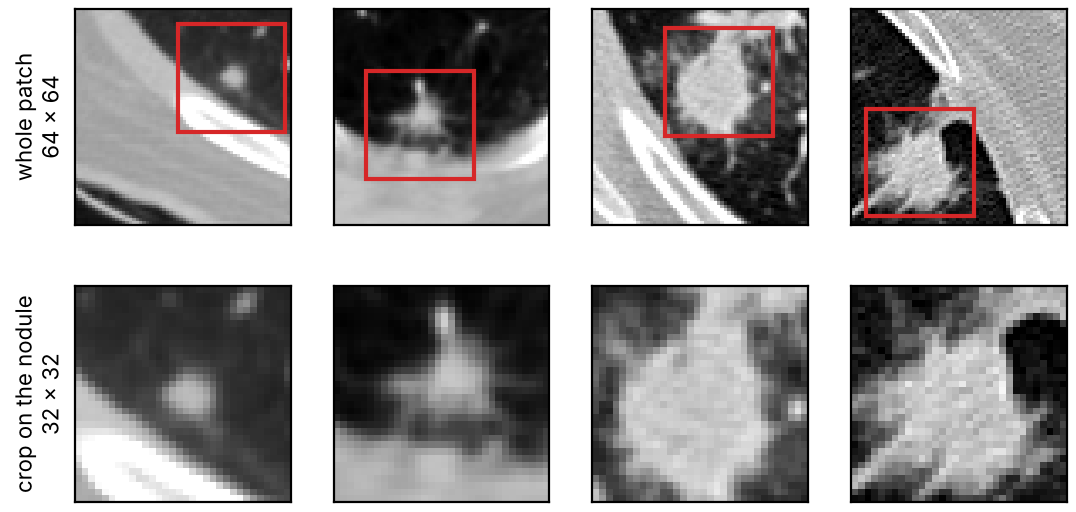
\includegraphics[width=0.6\linewidth]{fusion_crop.png}

{\small Four patients. Top: the whole patch, with the crop in red. Bottom: the $32 \times 32$ crop that the network sees.}
\end{center}

\textbf{What the network expects.} Our network was trained on colour photographs of $224 \times 224$ pixels, so
we do three things. We turn Hounsfield values into numbers between 0 and 1 (a window from $-1000$ to 400 HU). We
repeat the grey image in three equal channels. We enlarge it to $224 \times 224$ pixels and normalise it with the
mean and the standard deviation of ImageNet.

\textbf{Which numbers to keep.} A network produces many numbers per image, and we keep a summary. For a CNN such
as DenseNet121 we average the last feature maps: one number per map, 1024 in all. For a Vision Transformer we keep
either the \term{CLS token}, a special number list that the network builds to summarise the whole image, or the
mean of the patch tokens, one per small square of the image.

\textbf{How many numbers.} 1024 or 384 numbers are too many for 420 patients. We reduce them to 10 with a PCA.
The PCA finds the directions along which the embeddings vary most, and keeps the first ten. It learns from data,
so it is fitted on the training patients only. Fitted on all patients, it would already have seen the test images.

\textbf{Frozen or fine-tuned.} A frozen network is used as it is. A fine-tuned network continues to learn on your
images. We only use frozen networks, because fine-tuning needs many more patients than we have.

\textbf{2D or 3D.} We use one slice, so a 2D network. A 3D volume asks for a 3D network, such as Med3D, and more
memory.

\subsection{What we measured}

We tried six ways to turn the patch into numbers, with the same split and the same logistic regression as in the
notebook. The PCA to 10 components is fitted on the training patients. The column $R^2$ is a probe: a linear model
predicts the diameter of the nodule from the embedding, and we score it on the test patients (1 is perfect, 0 is
no better than the average). The last two columns give the AUC with the numbers alone, and together with the
clinical data (early fusion).

\begin{center}
\small
\begin{tabular}{@{}lrcrr@{}}
\toprule
Image numbers & Size & $R^2$ diameter & AUC alone & AUC with clinical \\
\midrule
Clinical data only & 4 & & 0.691 & \\
Five measurements from the mask & 5 & & 0.766 & 0.851 \\
DenseNet121 ImageNet, whole patch & 1024 & 0.385 & 0.724 & 0.796 \\
DenseNet121 ImageNet, crop on the nodule & 1024 & 0.587 & 0.741 & 0.843 \\
DINOv2 ViT-S/14 CLS, whole patch & 384 & 0.413 & 0.674 & 0.753 \\
DINOv2 ViT-S/14 mean of patches, whole patch & 384 & 0.384 & 0.681 & 0.754 \\
DINOv2 ViT-S/14 CLS, crop on the nodule & 384 & 0.595 & 0.763 & 0.852 \\
\bottomrule
\end{tabular}
\end{center}

\begin{center}
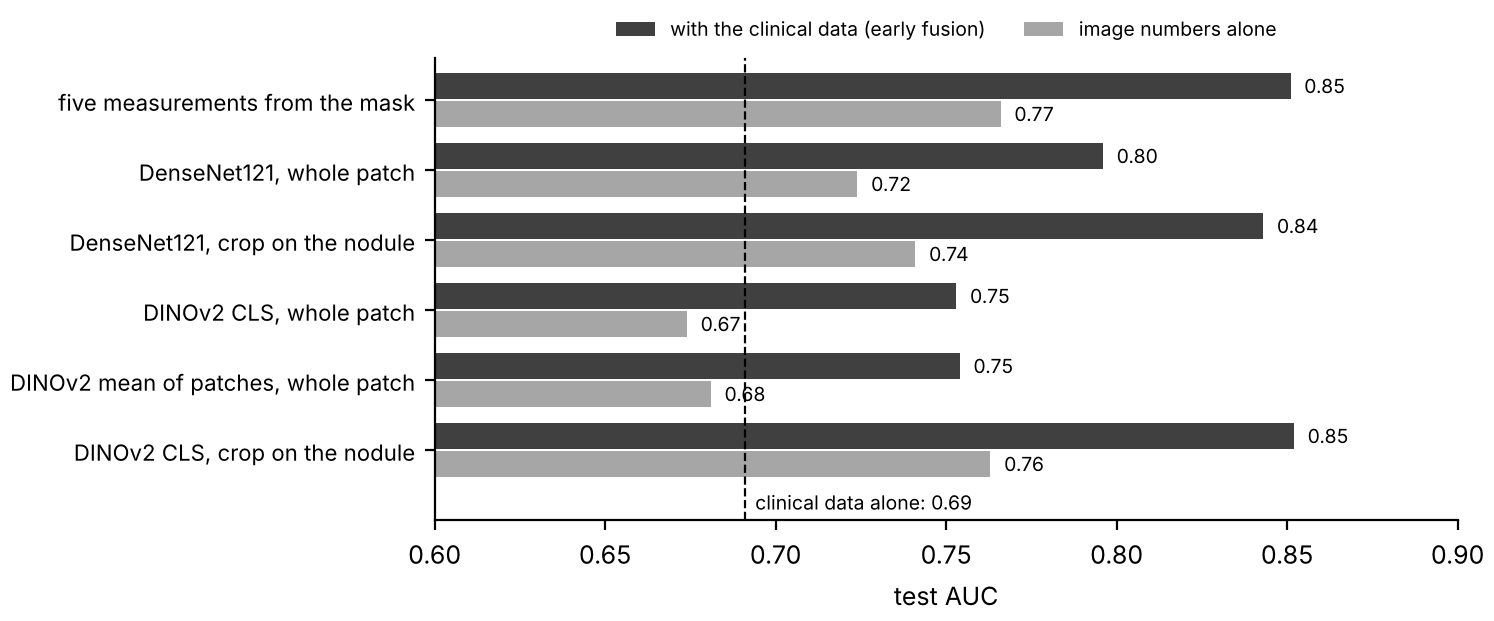
\includegraphics[width=0.7\linewidth]{fusion_embeddings.png}

{\small Test AUC of the same models. Dark: with the clinical data. Light: image numbers alone. The dashed line is the clinical data alone.}
\end{center}

What you can read in it:
\begin{itemize}
\item \textbf{Telling the network where to look matters more than which network.} With the crop on the nodule both
networks improve, alone and with the clinical data. DINOv2 on the crop reaches the level of the five measurements.
\item \textbf{Newer is not automatically better.} On the whole patch, DINOv2 is not better than the older
DenseNet121.
\item \textbf{CLS token or mean of the patch tokens:} no real difference here.
\item \textbf{The probe agrees with the task.} The embeddings that predict the diameter better ($R^2$ about 0.6 with
the crop, about 0.4 on the whole patch) are the ones that predict the outcome better. In our invented data the
outcome depends on the size, so this is expected. What matters is how you use a probe: a cheap check, before the
real task, that the embedding contains what you need.
\item \textbf{The crop uses the mask to find the centre.} In practice a detector, or a click of the radiologist,
gives it.
\item \textbf{One split, 181 test patients.} Differences of 0.02 or 0.03 are noise. The pattern ``the crop helps'' is
the only one large enough to trust.
\end{itemize}

These experiments are in the challenges at the end of the notebook. The complete code is in the file
\code{solutions/embedding\_comparison.py}.

\remember{An embedding is the list of numbers a pretrained network gives before its answer. Whether it helps
depends on how the network was trained, on what you show it, and on how many numbers you keep. Check it with a
probe and always compare it with the simple baselines.}

\further{
\item Bengio et al.\ \cite{bengio2013representation}: what a good representation is, in general.
\item Raghu et al.\ \cite{raghu2019transfusion}: does pretraining on photographs help for medical images?
\item Oquab et al.\ \cite{oquab2023dinov2}: the model we tested, designed to be used frozen.
}

% ===========================================================================
\parthead{Part III}{Putting the sources together}{Three places where image and table can meet, what the numbers say, and what happens outside the course.}

\section{Three ways to fuse}\label{c:6}
\usedin{notebook STEP 6, 7 and 9}

The three ways differ in one thing: \emph{where} the two sources meet. In the diagrams below grey boxes are
data, green boxes are models, and the white box is the place where the sources are joined. The three have the same
four columns, so you can compare them at a glance. We use the words of Huang et al.\ \cite{huang2020fusion}; other
authors use them a little differently \cite{cui2023fusionreview}.

\subsection{Early fusion}

The columns of the two sources are put side by side in one table, and \textbf{one} model learns from it
(STEP 6: \code{X\_early}).

\begin{center}
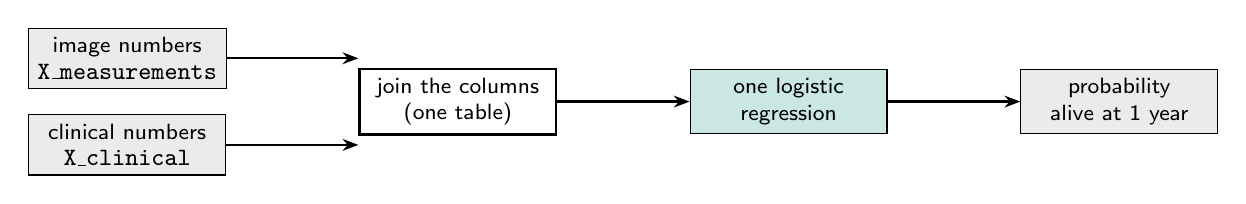
\begin{tikzpicture}
\node[dat] (a) at (0,0.55) {image numbers\\\code{X\_measurements}};
\node[dat] (b) at (0,-0.55) {clinical numbers\\\code{X\_clinical}};
\node[jn] (j) at (4.2,0) {join the columns\\(one table)};
\node[mod] (m) at (8.4,0) {one logistic\\regression};
\node[dat] (o) at (12.6,0) {probability\\alive at 1 year};
\draw[arr] (a) -- (j.west |- a);
\draw[arr] (b) -- (j.west |- b);
\draw[arr] (j) -- (m);
\draw[arr] (m) -- (o);
\end{tikzpicture}
\end{center}

\subsection{Late fusion}

Two models, each on its own data, and we combine their answers (STEP 7: the average of \code{p\_clinical} and
\code{p\_measurements}).

\begin{center}
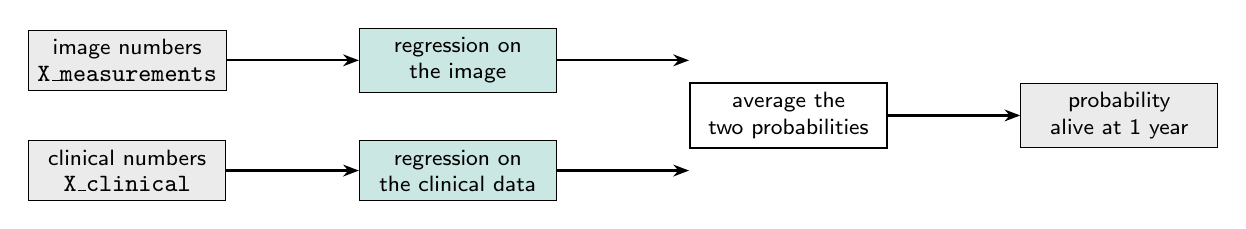
\begin{tikzpicture}
\node[dat] (a) at (0,0.7) {image numbers\\\code{X\_measurements}};
\node[dat] (b) at (0,-0.7) {clinical numbers\\\code{X\_clinical}};
\node[mod] (ma) at (4.2,0.7) {regression on\\the image};
\node[mod] (mb) at (4.2,-0.7) {regression on\\the clinical data};
\node[jn] (j) at (8.4,0) {average the\\two probabilities};
\node[dat] (o) at (12.6,0) {probability\\alive at 1 year};
\draw[arr] (a) -- (ma);
\draw[arr] (b) -- (mb);
\draw[arr] (ma) -- (j.west |- ma);
\draw[arr] (mb) -- (j.west |- mb);
\draw[arr] (j) -- (o);
\end{tikzpicture}
\end{center}

\subsection{Intermediate (joint) fusion}

One network with a branch for each source. The numbers of the two branches are joined inside the network, and the
image numbers are learned together with the final answer (STEP 9: \code{FusionNet}).

\begin{center}
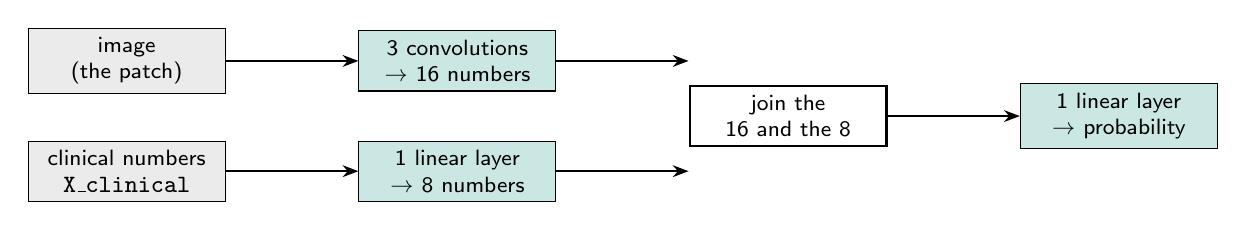
\begin{tikzpicture}
\node[dat] (a) at (0,0.7) {image\\(the patch)};
\node[dat] (b) at (0,-0.7) {clinical numbers\\\code{X\_clinical}};
\node[mod] (ma) at (4.2,0.7) {3 convolutions\\$\to$ 16 numbers};
\node[mod] (mb) at (4.2,-0.7) {1 linear layer\\$\to$ 8 numbers};
\node[jn] (j) at (8.4,0) {join the\\16 and the 8};
\node[mod] (m) at (12.6,0) {1 linear layer\\$\to$ probability};
\draw[arr] (a) -- (ma);
\draw[arr] (b) -- (mb);
\draw[arr] (ma) -- (j.west |- ma);
\draw[arr] (mb) -- (j.west |- mb);
\draw[arr] (j) -- (m);
\end{tikzpicture}
\end{center}

\subsection{Comparison}

\begin{center}
\small
\begin{tabular}{@{}>{\raggedright\arraybackslash}p{2.4cm}>{\raggedright\arraybackslash}p{3.2cm}>{\raggedright\arraybackslash}p{1.7cm}>{\raggedright\arraybackslash}p{3.0cm}>{\raggedright\arraybackslash}p{3.6cm}@{}}
\toprule
 & What is joined & Models & What it needs & When it is handy \\
\midrule
Early & the input columns & one & both sources for every patient & few patients, simple model, quick to build \\
Late & the output probabilities & two & each model needs only its own source & a source is missing for some patients, or two teams built the models \\
Intermediate & numbers inside a network & one network & many patients, or a pretrained branch & you want the image numbers learned for the task \\
\bottomrule
\end{tabular}
\end{center}

In a review of 34 studies, early fusion was the most used, in 22 of the 34 \cite{mohsen2022fusion}. That tells
you what people do, not what works best.

\remember{Early joins the inputs, late joins the answers, intermediate joins the numbers in the middle. None is
the best in general: it depends on the data you have.}

\further{
\item Huang et al.\ \cite{huang2020fusion}: the systematic review whose words we use.
\item Cui et al.\ \cite{cui2023fusionreview}: another review, on image and non-image data for diagnosis and prognosis.
\item Mohsen et al.\ \cite{mohsen2022fusion}: a review that counts which fusion is used.
}

% ---------------------------------------------------------------------------
\section{Reading the results}\label{c:7}
\usedin{notebook STEP 10}

\begin{center}
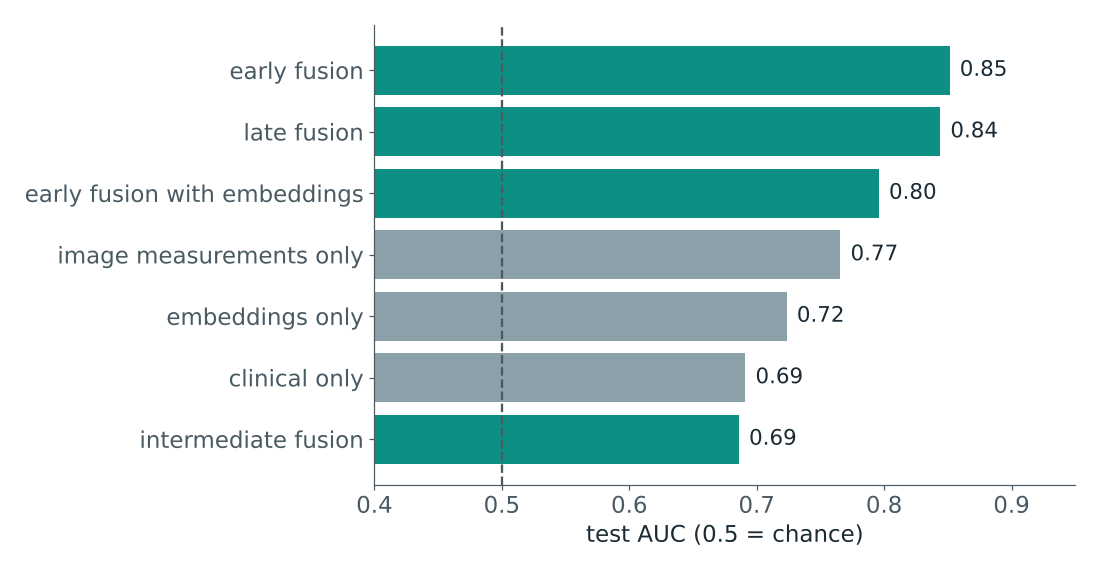
\includegraphics[width=0.62\linewidth]{fusion_results.png}

{\small Test AUC of the seven models (one split, 181 test patients). Grey: one source. Green: fusion.}
\end{center}

Early fusion (0.851) and late fusion (0.844) beat both baselines, clinical only (0.691) and image measurements
only (0.766). Each source knows something the other does not: the table knows age, smoking and performance
status, the measurements know size and density. Early fusion with embeddings (0.796) is better than the clinical
data alone but worse than fusion with the measurements, as the embeddings are the weaker image model (0.724). The
intermediate network (0.686) is no better than the clinical data alone: with 420 patients it has too little data
to learn the image numbers from scratch. Chapter 5 showed that a crop on the nodule closes most of the gap
between embeddings and measurements.

\textbf{What to be careful about.}
\begin{itemize}
\item \textbf{The data are invented.} The formula was built so that both sources matter, so fusion is almost
guaranteed to help. On real data it often helps less: the image and the table frequently tell the same thing.
\item \textbf{The test set is small.} With 181 patients a difference of 0.02 or 0.03 between two models is noise.
Change \code{random\_state} and watch the ranking move.
\item \textbf{Fit everything on the training patients.} The scaler and the PCA learn from data, so they are fitted
on the training patients only, and then applied to the test patients.
\item \textbf{Alive at one year is a simplification.} Yes or no ignores the patients lost before one year and the
time of death. Such patients are \term{censored}: we know they were alive until a certain day, not after. Real
studies use survival analysis \cite{clark2003survival}.
\end{itemize}

\remember{Compare every fusion with the best single source, on the same test patients, and do not read
differences smaller than 0.03 on 181 patients.}

\further{
\item Clark et al.\ \cite{clark2003survival}: the basic concepts of survival analysis, including censoring.
\item Kapoor and Narayanan \cite{kapoor2023leakage}: why results that look good may not hold.
}

% ---------------------------------------------------------------------------
\section{Outside this notebook}\label{c:8}
\usedin{reading}

\textbf{A real example.} A study on lung screening CT combined the image with clinical data
\cite{gao2021lungfusion}. With about 23\,500 patients the AUC was 0.88 for the fused model, 0.86 for the image
only and 0.69 for the clinical data only. The gain over the image alone was small, and that is the usual size of a
real gain. Compare it with our invented case, where the gain was large.

\textbf{Foundation models and images with text.} The idea of chapter 5 is growing. Large models trained on huge
sets of images, and on images with their text, are used as ready-made encoders for medicine
\cite{zhang2023biomedclip,zhou2023foundation,pai2024foundation}. The three schemes of chapter 6 apply there too.

\textbf{Where the field is going.} Reviews describe the open questions of multimodal medicine and of multimodal
machine learning in general \cite{acosta2022multimodal,liang2024foundations}.

\textbf{Course material.} The CMU course on multimodal machine learning \cite{cmummml} and the MONAI tutorials
\cite{monaidocs} have lectures and code you can run.

\remember{Real gains from fusion are usually modest. Ready-made encoders trained on images and text are the
direction of the field.}

\further{
\item Gao et al.\ \cite{gao2021lungfusion}: the lung screening study with the numbers above.
\item Liang et al.\ \cite{liang2024foundations}: principles and open questions of multimodal learning.
\item CMU 11-777 \cite{cmummml} and the MONAI tutorials \cite{monaidocs}: free material, with code.
}

% ---------------------------------------------------------------------------
\clearpage
\phantomsection\label{c:refs}
{\footnotesize
\bibliographystyle{unsrt}
\bibliography{references}
}

% ---------------------------------------------------------------------------
\section*{Index of terms}\label{c:index}

\begin{center}
\small
\begin{tabular}{@{}lcp{9.2cm}@{}}
\toprule
Term & Chapter & In one line \\
\midrule
AUC & 3 & probability that an alive patient scores higher than a patient who was not; 0.5 chance, 1 perfect \\
Baseline & 3 & a model on one source only, the one fusion must beat \\
Censoring & 7 & a patient followed only up to a date, then lost \\
CLS token & 5.5 & the number list a Vision Transformer builds to summarise the whole image \\
Crop & 5.5 & a smaller piece of the patch, centred on the nodule \\
Early fusion & 6 & join the columns, train one model \\
Embedding & 5.1 & the list of numbers a pretrained network gives just before its answer \\
Fine-tuning & 5.5 & continue to train a pretrained network on your images \\
Foundation model & 8 & a large model trained on huge data, used as a ready-made encoder \\
Frozen network & 5.1, 5.5 & a pretrained network used as it is, without training \\
Fusion & 1 & one model that uses several modalities \\
Image and text recipe & 5.3 & matching image and caption get close embeddings \\
Intermediate (joint) fusion & 6 & one network, one branch per source, joined inside \\
Late fusion & 6 & one model per source, join the answers \\
Leakage & 3 & information from the test patients reaching the training \\
Mask & 4 & the outline of the nodule, drawn by a person or a program \\
Modality & 1 & one kind of data: image, table, text \\
PCA & 5.5 & keeps the few directions along which the data vary most \\
Pretrained network & 5.1 & a network already trained on a large dataset \\
Probe & 5.2, 5.6 & a simple model that tries to read a known property from the embedding \\
Radiomics & 4 & describing a lesion with numbers of shape, intensity and texture \\
Representation learning & 5.1 & learning the list of numbers that makes the next task easy \\
Self-supervised & 5.3 & learning without labels, from two views of the same image \\
Supervised & 5.3 & learning to give a label written by a person \\
Vision Transformer (ViT) & 5.3, 5.4 & a network that cuts the image into small squares and reads them as a sequence \\
\bottomrule
\end{tabular}
\end{center}

\end{document}
